\begin{flushright}
    تابع f از Rn به R را محدب میگوییم اگر به ازای هر x,y عضو Rn و هر $\theta$ بین 0 و 1:



    \begin{displaymath}
        f(\theta x + (1-\theta)y) \leq \theta f(x) + (1-\theta)f(y)
    \end{displaymath}

    \begin{figure}[H]
        \centering
        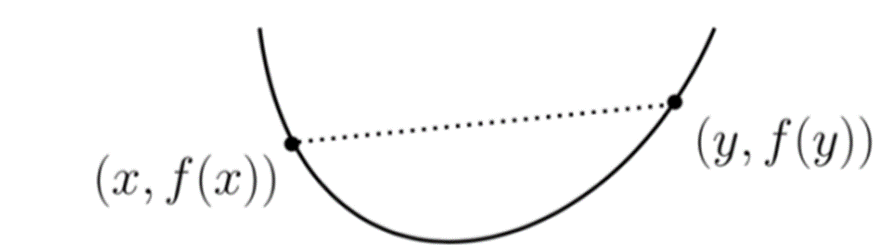
\includegraphics[width=0.8\textwidth]{source/convex-function.png}
        \label{fig:convex}
    \end{figure}


    می توان نشان داد یک تابع محدب است اگر و تنها اگر مشتق دوم آن مثبت باشد (در ابعاد بالاتر ماتریس هسین مثبت نیمه معین باشد). (اثبات اسلاید 15)

    مجموعه ای را محدب میگوییم اگر به ازای هر خط گذرنده بین 2 عضو در این مجموعه تمامی نقاط این خط نیز عضو مجموعه محدب باشد.
    \begin{figure}[H]
        \centering
        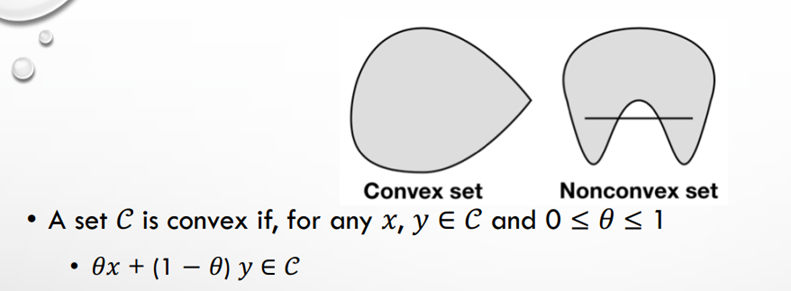
\includegraphics[width=0.8\textwidth]{source/convex-set.png}
        \label{fig:convex-set}
    \end{figure}

    نکته مهم توابع محدب این است در این توابع بهینه محلی همان بهینه جهانی است.
     در نتیجه پیدا کردن بهینه محلی منجر به minimize کردن تابع هدف میشود.

    \begin{figure}[H]
        \centering
        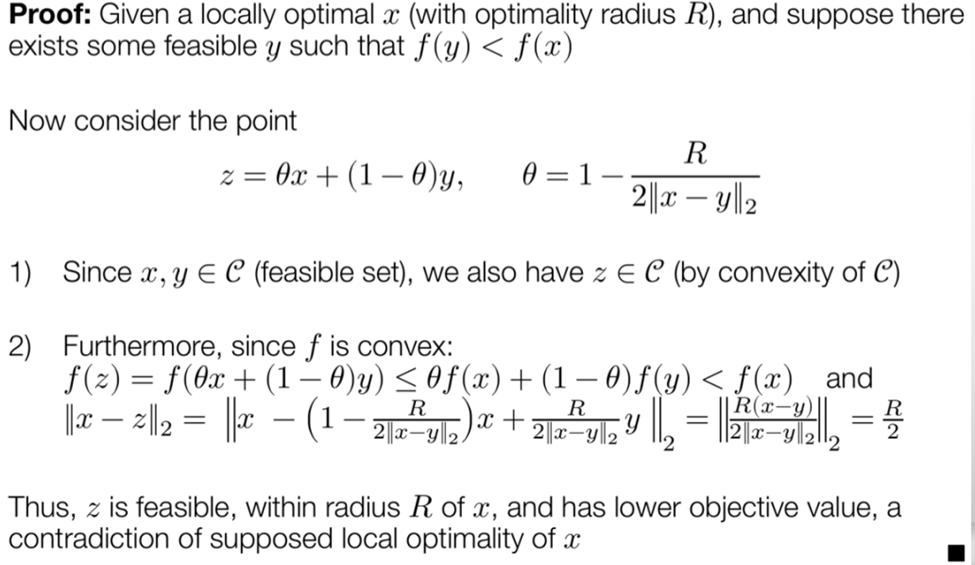
\includegraphics[width=0.8\textwidth]{source/global-min-in-convex.png}
        \label{fig:convex-example}
    \end{figure}

\end{flushright}